%-------------------------------------------------------------------------------
\documentclass[11pt]{article}

\usepackage{amsmath} 
\usepackage{amsfonts}
\usepackage{amssymb}
\usepackage{booktabs}
\usepackage[usenames, dvipsnames]{color} 
\usepackage{dsfont}
\usepackage{epigraph}
\usepackage{graphicx}
\usepackage{hyperref}
\usepackage[utf8]{inputenc}
\usepackage{lscape}
\usepackage{natbib}
\usepackage{setspace}
\usepackage{subfig}


\bibpunct{(}{)}{;}{a}{,}{,}

\setlength{\oddsidemargin}{0 in}
\setlength{\evensidemargin}{0 in}
\setlength{\textwidth}{6.3 in}
\setlength{\textheight}{8.6 in}
\setlength{\topmargin}{-.6in}
\setlength\parindent{0.25in}
\setlength\parskip{0.25in}

\hypersetup{                                                                                                    
    colorlinks=true,   
    linkcolor=BlueViolet,
    citecolor=BlueViolet,
    filecolor=BlueViolet,
    urlcolor=BlueViolet
}  

%-------------------------------------------------------------------------------


%-------------------------------------------------------------------------------
\begin{document}

\title{{\bf\Large{\textsl{Maternal Mortality and Female Life Expectancy: }\\ \large\normalsize The Importance of Gender Inequality}} \footnotemark[7] 
\author{Sonia Bhalotra\\ \normalsize{University of Essex}\footnotemark[1] \and Damian Clarke\\ \normalsize{University of Oxford}\footnotemark[2]\\ \and Joseph Gomes\\ \normalsize{University of Essex}\footnotemark[3]\\\\ \and Atheendar Venkataramani\\ \normalsize{Massachusetts General Hospital}\footnotemark[4]\\}}

\date{\today}


\renewcommand{\thefootnote}{\fnsymbol{footnote}} % makes footnotes as symbols

\footnotetext[1]{\noindent ISER \& Department of Economics, University of Essex, Wivenhoe Park, Colchster CO4 3SQ, United Kingdom, \texttt{ e-mail: 
\href{mailto:srbhal@essex.ac.uk}{srbhal@essex.ac.uk}}}


\footnotetext[2]{Department of Economics, University of Oxford, UK \texttt{ e-mail:
\href{mailto: damian.clarke@economics.ox.ac.uk}{ damian.clarke@economics.ox.ac.uk}}}

\footnotetext[3]{\noindent ISER, University of Essex, Wivenhoe Park, Colchster CO4 3SQ, United Kingdom, \texttt{ e-mail: 
\href{mailto:jgomes@essex.ac.uk}{jgomes@essex.ac.uk}}}

\footnotetext[4]{Masachusstes General Hospital, USA \texttt{ e-mail: 
\href{mailto:avenkataramani@partners.org}{avenkataramani@partners.org}}\\ \vspace{0.5cm}}

\footnotetext[7]{We are grateful to all seminar participants in the FRG seminar at ISER, Essex, NEUDC 2014 conference in Boston University,  Growth Conference in ISI Delhi Dec 2014, and RES 2015 in Manchester, for their comments and feedback.}


\thispagestyle{empty}
\maketitle
\renewcommand{\thefootnote}{\arabic{footnote}} \setcounter{footnote}{0} 



\begin{abstract}
Societies with higher levels of gender inequality are slower and less likely to
address women-specific health outcomes.  We demonstrate this by examining 
maternal mortality ratios (MMR) and the gap between women's and men's life 
expectancy.  We show that socities that are more gender predjudiced 
have higher levels of maternal mortality, slower rates of reduction of maternal 
mortality, and life expectancy differentials \emph{less} favourable for women.
This holds conditional on country income.  In terms of maternal mortality 
reductions, a 1 standard deviation (sd) reduction in gender predjudice is 
equivalent to a xx.xx-xx.xx sd increase in log(GDP).  Despite these large effects
on women's health, our various measures of gender predjudice are shown to have 
no significant effect on TB infection rates---a gender neutral illness which we 
consider as a placebo test.  Using historical data from the USA, we show that
this phenomenon can be partially explained by the fact that areas with higher 
levels of gender equality are less willing (or able) to apply available 
technologies to improve female-specific health outcomes.
\end{abstract}

\emph{JEL codes:} I14, I15, O15. 

\thispagestyle{empty}
\setlength{\baselineskip}{1.4\baselineskip} 
\newpage 
\begin{spacing}{1.4}

%-------------------------------------------------------------------------------
\section{Introduction}
\epigraph{`\textit{`In some regions of the world inequality between women and 
men directly involves matters of life and death, and takes the brutal form of 
unusually high mortality rates for women...}'' }{\citet{sen2001many}}

In September of 2000, all 189 UN Member States committed to addressing 8 
Millennium Development Goals.  One of these goals (goal 5A) was to reduce by 
three quarters the maternal mortality ratio (MMR) between 1990 and 2015.  Today 
in 2015, the most recent measures suggest that MMR is 55\% (rather than 25\%) 
what it was in 1990. However, progress towards other goals has been closer to 
target. The world-wide rate of child mortality has fallen 50\% since 1990: far 
closer to the stated aim of a two-thirds reduction.\footnote{Measures of child 
mortality and MMR come from the World Bank Data Bank (measures SH.DYN.MORT and 
SH.STA.MMRT respectively).  The most recent year available for each measure is 
2013.  According to this data, World MMR has fallen 380 per 100,000 live births 
to 210 per 100,000 births, while under 5 mortality has fallen from 90.2 per 
1,000 live births to 45.6 per 1,000.}  In this paper we examine whether the 
relatively anemic progress towards goal 5A, and female health outcomes more 
generally, is because MMR is a \emph{woman} specific outcome, which gender-% 
predjucided states are less likely to address.

Prevailing popular logic suggests that an increase in investment levels will 
lead to a reduction in maternal deaths (Lancet, Gates cite).  The results of 
this paper suggest that investment alone is not enough.  We demonstrate that 
cultural change, specifically preferences towards women's rights is a 
fundamental determinant of women's health.  By various measures, a 1 sd 
reduction in the level of gender predjudice is as important as a xx sd increase 
in country income levels.

%Using country by year 


The female-specific disease burden from MMR is a considerable problem for public 
health and economic and social well-being.  MMR has fallen sharply in the last 
decade, but still remains unnecessarily high, at around 800 deaths a day. In 2013 
alone, around 289,000 women died due to pregnancy or child birth related 
complications \citep{WHO2014}. Almost all these deaths (99\%) are concentrated 
entirely in developing countries. The average MMR in low income countries in 2010 
was estimated to be 452 deaths per 100,000 births, similar to the rates that 
prevailed in England and Wales in 1930 before the introduction of antibiotics.%
\footnote{452 per 100,000 is the average MMR for the 35 low income countries 
(World Bank classification). The MMR for England and Wales was 440, for Denmark 
it was 380 and for the US it was 673 in the year 1930 \citep{loudon1992death}.} 
This is pertinent given that 40-50\% of maternal deaths are on account of 
post-partum puerperal sepsis which is treatable with antibiotics. Infant 
mortality, which is also largely determined by infectious disease, claimed policy 
attention much earlier and, apparently with more commitment. 



%-------------------------------------------------------------------------------
\section{Data and Descriptive Statistics}
\subsection{Data}
\label{scn:data}
Our data comes from a wide range of sources: both at the macro (country$\times$%
year) level, as well as microdata from household suveys conducted in a large
number of countries.  This allows us to construct measures of health outcomes
(both women-specific and gender-neutral), as well as gender predjudice measures
(described below).  These are measured from 1960-2013, although important gaps
exist in the case of some variables.

Health outcome variables come directly from the World Bank data bank. These 
include female and male life expectancy (in years), the maternal mortality ratio 
(deaths per 100,000 live births), tuberculosis rates (incidence per 100,000 
people), as well as GDP, which we use as a covariate.  These variables are 
recorded yearly from 1960 to 2013, with the exception of MMR, which is recorded 
quinquennially from 1990 to 2010 (inclusive).  Summary statistics for these 
variables are included in panel A of table \ref{TAB:sumstats}.  We use age-%
specific mortality rates for women and men which are supplied by 
\citet{UNMortality2012}.  These are also available quinquennially, however 
starting in 1960 and ending in 2005.  Additional details of these (and all) 
variables are provided as a data appendix \ref{app:Data}.

Measures of gender predjudice are obtained and calculated from a wide range of
sources.  These include measures of women's rights, measures of female 
representation in national legislatures and parliaments, gender bias inherent
in majority spoken languages, and measures of parental bias towards the 
preferred gender of their children.

Women's right measures are collected from a previously under-exploited cross-%
country rights dataset \citep{CingranelliData2013}, which provides data on three 
different variables measuring political, economic and social Rights of women for 
the period of 1981 to 2011 for around 127 (in 1981) to 192 (in 2011) countries.
A discussion of the construction of these variables are included in the data
appendix, and summary statistics are provided in table \ref{TAB:sumstats}.  To
examine women's political represenation, we use data from the World Bank data bank
which measures ``Proportion of seats held by women in national parliaments (\%)''.
This is available for between 160 to 188 countries (depending on the year) for 
the period of 1997--2013.

Gender intensity of language measures are designed to capture the influences which
spoken and written language has gender attitudes and outcomes in society.  Recent
work has demonstrated that gender salience embedded in languages are correlated 
with a range of gender outcomes including maternity leave policy differences across 
countries \citep{givati2012law}, and female labour force and political 
participation \citep{gay2013}. For gender salience of languages we use the data and 
classification of \cite{gay2013} and \citet{givati2012law}, both of which focus on
the female/male distinctions in grammar.  \citet{givati2012law} use the number of 
cases of gender differentiated pronouns for 33 languages as a measure of gender 
neutrality of the language, while \cite{gay2013} use the gender related grammatical 
variables coming from the World Atlas of Linguistic structures and have four binary 
variables related to gender neutrality of languages.  These are a Sex-Based Intensity 
Index, Number Gender Intensity Index, Gender Assignment Intensity Index, Gender 
Pronouns Intensity Index, as well as a Gender Intensity index (GII) which is a sum of 
all these four indices.  Further details regarding the construction of these variables 
are provided in appendix \ref{app:Data}.

Finally, we aggregate an individual-specific measure of gender bias from a 
series of widely applied household surveys to the country$\times$year level. In 
the Demographic and Health Surveys (DHS) each surveyed woman is asked about her 
ideal number of children, ideal number of boys, and ideal number of girls. Using 
these stated preferences we construct the society-level desired sex ratio (DSR) 
calculated by dividing the desired number of boy children by the desired number 
of girls.  In this case a higher DSR implies more biased gender preferences of 
mothers.

%-------------------------------------------------------------------------------
\subsection{Descriptive Statistics and Unconditonal Correlations} 
The last five decades have witnessed large and sustained increases in the life 
expectancy rates at birth for both men and women throughout the world. Typically 
women have enjoyed a life expectancy advantage over men in almost all countries 
of the world. However, some interesting cross country differences exist in the 
data. In particular, there are two striking features that emerge from studying 
life expectancy advantage of women over men in the developing world. First, when 
the AIDS epidemic struck Africa in the 1990s, women lost more in terms of life 
expectancy than men and with a corresponding reduction in life expectancy 
advantage. However, with the arrival of anti-retro viral treatment in the mid 
2000s onwards, the female advantage in life expectancy started to go up yet 
again (See Figure \ref{SSALEtrend}).\footnote{See 
\url{http://www.who.int/gender/hiv_aids/en/} for a discussion on gender and 
AIDS.} Second, in contrast to not only all other parts of the world but also to 
sub-Saharan Africa, women actually started with a life expectancy disadvantage 
in South Asia (See Figure~\ref{SASLEtrend}). This is not surprising given that 
South Asia is know to be more gender prejudiced than other regions of the world. 
Only since the 1980s has the life expectancy of women exceeded that of men, 
a trend that has increased over time.

In turning to \emph{correlations} between life expectancy and country income
levels, figure \ref{lLEGDP} plots female life expectancy against GDP. In each 
panel (decade) of this figure, female life expectancy has a positive relation 
with GDP. A similar picture emerges when plotting male life expectancy against 
GDP.\footnote{See the scatter plots in \ref{ScatterFLE} for example.} This is 
not surprising and has been well documented in the literature. However, 
strikingly, once we plot the female life expectancy advantage i.e. the log 
ratio of female to male life expectancy against GDP in Figure \ref{lLErGDP0}, we 
see that relationship nearly disappears. While the link between health outcomes
and country income level is strong, gender gaps in health outcomes have a much
weaker correlation with country income.

Turning to maternal mortality ratios (maternal deaths per 100,000 live 
births), existing data suggests a recent downward trend since the 1990s.  
However, while the maternal mortality ratio (MMR) has been sharply declining for 
the world as a whole, there is considerable variation across regions, and, 
according to some estimates, the decline has been sharp only in the post 2003 
period after a much slower rate of change in the earlier decades.\footnote{It is 
important to note the difficulty in accurately measuring MMR 
\citep{hogan2010maternal,kassebaum2014global}. Here we generally work with WHO 
estimates documented in \citet{hogan2010maternal}, however also construct our 
own alternative estimates based on the sisterhood method \citep{Grahametal2008} 
using DHS micro-data.}  Despite the sharp fall in the 2000s (see figure 
\ref{fig:MMRRegion} for trends by region), only 16 countries, seven of which are 
developing, are expected to achieve the MDG of reducing MMR by 75\% by the year 
2015 \citep{kassebaum2014global}.  

Finally, we plot unconditional correlations between female-specific health 
measures and gender-predjudice varaibles across countries.  Graphs by year, 
and also pooled over time provide descriptive evidence that countries with
worse female-specific health outcomes are also those which are more gender-biased.
Figure \ref{LFEgenderbias} displays female life expectancy and female life 
expectancy advantage against the country average desired sex ratio of children.
While life expectancy is negatively related to DSR (ie more biased countries
have lower life expectancies), the negative correlation with life expectancy 
advantage appears to be even more negative.  Similarly, for both DHS measures
of MMR (figure \ref{MMRDgenderbias}) and WDI measures (figure 
\ref{MMRWgenderbias}), more biased countries (as proxied by DSR) have higher
rates of maternal death in childbirth.

%--------------------------------------------------------------------------------
\section{Methodology}
\label{scn:methodology}
\subsection{Gender Preferences and Women's Health}
We test our prevailing hypothesis that gender-biased preferences drive female-%
specific health outcomes.  To do so, we begin by estimating the following 
regression using the panel data described in the previous section:
\begin{equation}
\label{eqn:panel}
FemaleHealth_{it} = \alpha + \beta GenderBias_{it} + \gamma_i + \delta_t + 
               (\phi_i\times t) + \theta X_{it} + \varepsilon_{it}.
\end{equation}
Here $FemaleHealth_{it}$ is a measure of health stocks or outcomes speficic 
to women in country $i$ and time $t$.  As discussed in section X.X,
female health is measured in two ways: using a female-specific mortality measure
(MMR), and using a relative measure of female health stocks to male health stocks 
(LE advantage).  We include country-specific fixed effects $\gamma$, and year 
specific fixed effects $\delta$ while allowing for differential trends in female 
health measures by country.  Standard errors are always clustered at the level
of the country.

Consistent estimates of $\beta$---the effect of gender-biased preferences on
female health---requires that the transitory error term $\varepsilon_{it}$
contains no factors correlated with both our measure of gender bias and female 
health outcomes.  While in our most demanding specifications we include a 
number of time-varying controls $X_{it}$ (including levels and growth of GDP), 
it is unlikely that observable 
measures will capture all time varying country-specific factors which affect
both variables.  As such, we view (\ref{eqn:panel}) as compelling descriptive 
evidence, and later employ a number of alternative specifications, methodologies 
and falsification tests which allow us to reach causal conclusions regarding the 
effect of gender bias on female health.  We describe these tests in the following 
sections 

\subsubsection{Measuring Gender Bias}
\label{ssscn:gendbias}
In our most na\"ive regressions, we use a range of accepted measures of gender
bias as our independent variable in (\ref{eqn:panel}).  Different measures are 
collected at the level of the individual, or the level of the country, and in
each case, vary over time and space.  These initial variables are: desired sex
ratio; the Cingranelli et al.\ political, economic and social rights of women
measures; and proportional representation of women in national parliaments. We
provide additional descriptive statistics and discussion of these variables in 
section \ref{scn:data}.

In each case we progressively control for $\log($GDP$)$, and an interaction 
between $\log($GDP$)$ and our independent variable of interest.  We thus 
estimate the effect of gender bias on woman-specific health outcomes conditional 
and unconditional on country income levels, to allay concerns that both gender 
bias and outcomes such as MMR are jointly driven by country income.

%-------------------------------------------------------------------------------
\subsubsection{Predetermined Measures of Gender Bias}
\label{ssscn:language}
Measures of gender bias used in estimation up to this point are (either directly 
or indirectly) based on contemporaneous decisions by a society and/or its 
members.  Thus, even controlling for time-varying covariates, trends and fixed 
effects, endogeneity concerns still exist.  Given these concerns, we focus on a 
measure of gender attitudes which is entirely pre-determined, and arguably 
entirely exogenous when considering contemporaneous maternal mortality and life 
expectancy advantage.

Following Givati and Troiano (2012) and Gay et al.\ (2013), we use measures of
the inherent gender neutrality (or gender bias) built into the grammatical 
structure of different languages.\footnote{These authors suggest that grammatical 
gender can influence and reflect gender attitudes in society and are correlated 
with different gender outcomes including maternity leave policy differences 
across countries (Givati and Troiano, 2012), female labour force participation, 
and political 
participation (Gay et al., 2013). Language grammar was established centuries in 
the past and is one of the features of language that is stable over long periods 
of time. Moreover, grammatical gender is something that an individual is born 
in to and thus arguably a more exogenous measure of gender bias in society.}  We 
estimate:
\begin{equation}
\label{eqn:gii}
FemaleHealth_{it} = \beta_0 + \beta_1 GII_i + \beta_2 PercentLang_i + X_{it} + X_i 
                  + \nu_{it},
\end{equation}
where $FemaleHealth_{it}$ is identical to that described in model 
(\ref{eqn:panel}). Here, $GII$, (Gender Intensity Index), refers to the measure 
of the gender bias inherent in the language, as coded by Givati and Troiano, and 
Gay et al.  Precise details regarding this variable are provided in section X.X 
and appendix X).

Given that the language of country $i$ is essentially fixed over time, we can no
longer include country fixed effects, as these capture (among other things) the
language spoken in the country.  We thus now control for both fixed ($X_{i}$) 
and time varying ($X_{it}$) country-level variables, including decade dummies, 
continent dummies, $\log($GDP$)$, the log of population, religion, income and 
climate factors.  Finally, given that $GII$ is defined based on the majority
language in each country, we control for the percentage of inhabitants of each
country which speak the particular language.

\subsubsection{Falsification Tests: Gender Neutral Disease Burden}
\label{ssscn:TB}
The analysis discussed so far in this section tests the hypothesis that gender
biased preferences slow the improvement of female-specific health outcomes 
(namely maternal mortality, and relative life expectancy).  In order to provide
evidence that it is indeed \emph{female}-specific health outcomes which are 
driven by gender preferences, we run a series of falsification tests.  These
falsification tests consist of estimating the previous regressions, however 
focusing on a gender-neutral health outcome.

We thus focus on rates of tuberculosis (TB) infection.  TB is a gender-neutral
condition\footnote{According to the WHO ``In most of the world, more men than 
women are diagnosed with tuberculosis (TB) and die from it. TB is nevertheless 
a leading infectious cause of death among women.''}, %http://www.who.int/tb/challenges/gender/en/
 and was the second most common infectious cause of death world wide in 2014 
(WHO, 2015). %http://www.who.int/mediacentre/factsheets/fs104/en/
Given that it affects individuals indiscriminately by gender, it is a
 particularly suitable placebo for our analysis.  Based on this placebo, we 
estimate analogues to (\ref{eqn:panel}) and (\ref{eqn:gii}).  For example, for 
(\ref{eqn:panel}) we estimate:
\begin{equation}
TB_{it} = \alpha^{TB} + \beta^{TB} GenderBias_{it} + \gamma^{TB}_i + \delta^{TB}_t + 
               (\phi^{TB}_i\times t) + \theta^{TB} X_{it} + \varepsilon^{TB}_{it},
\end{equation}
and if $\hat\beta$ but not $\hat\beta^{TB}$ is significantly (and economically)
significant, this lends support to the hypothesis that gender preferences halt
progress on (only) woman-specific conditions.


\subsection{Testing Mechanisms}
After documenting the effect that gender-biased preferences have on female
health outcomes, we turn to testing the mechanisms that drive these results.
Using the arrival of sulfanide drugs (the first antibiotics) to the United 
States in 1937, we test whether states which were early to legislate suffrage 
were more likely to adopt medical technologies which could be employed to 
directly reduce rates of maternal mortality. We define early legislators of 
suffrage as those states which passed suffrage laws prior to the mandated 
national reform in 1920.  Using these two groups of states, we follow 
Jayachandran et al.\ (2010) and estimate the following difference-in-differences 
specification around the 1937 date of arrival of sulf drugs:
\begin{eqnarray}
\label{eqn:sulfa}
log(MMR)_{st} & = \alpha + \beta \mathds{1}[Post1937]_t + \gamma(EarlySuf_{s}\times t)
                + \delta_1 (EarlySuf\times Post1937_t) \nonumber \\
              & + \delta_2 (EarlySuf\times Post1937_t\times t) + \phi_t + \mu_s
                + \upsilon_{st}.
\end{eqnarray}
In these regressions we always weight states ($s$) by their population, and 
cluster standard errors at the level of the state.

By estimating (\ref{eqn:sulfa}), we are able to split the quantitatively 
important (exogenous) 
reduction in maternal deaths which occurred with the arrival of the first 
antibiotics into three components.  The first, $\beta$, identifies the immediate 
general effect of sulfanide drugs on MMR, while $\delta_1$ and $\delta_2$ test 
whether there are larger level and trend breaks (respectively) in states that 
were early adopters of women's suffrage, and which presumably had long-standing 
norms evolving in favor of women's autonomy.

Sulfa drugs were also important in reducing morbidity and mortality from 
pneumonia.  Unlike maternal mortality, pneumonia mortality affects males 
more than females, and infants in particular.  Thus, as in section 
\ref{ssscn:TB}, we employ a similar logic, and use rates of pneumonia (for 
which there is also a post-1937 trend break), as a falsification test.  We 
restimate (\ref{eqn:sulfa}), replacing maternal mortality with pneumonia 
mortality as our dependent variable.  Our placebo test is based on the 
coefficients $\delta_1$ and $\delta_2$.  If states with a lower preference for 
female equality invest less (only) in applying available technologies to 
female-specific illnesses, then $\delta_1$ and $\delta_2$ should be negative in 
(\ref{eqn:sulfa}), but not significant in the gender-neutral pneumonia version
of (\ref{eqn:sulfa}) estimated for pneumonia rather than MMR.

%-------------------------------------------------------------------------------
\section{Results}
\subsection{Female Health and Gender Predjudice}


\subsection{Gender Intensity of Language}
Language grammar was established centuries in the past and is one of the 
features of language that is stable over long periods of time. Moreover, 
grammatical gender is something that an individual is born with and thus 
arguably a more exogenous measure of gender bias in society.


\subsection{US Case Study: Early Suffrage, Adoption of Medical Technology, and 
Maternal Mortality}
In order to examine the \emph{mechanisms} which drive the relationship between
gender bias and excessively poor female health outcomes we explore a historical
case study.  We focus on the interplay between early suffrage and the post-1937 
fall in maternal mortality driven by the arrival of the first antibiotics in 
the United States. Women's suffrage was institutionalized at the national level 
in 1920 with the 19\textsuperscript{the} amendment to the U.S. Constitution. 
However, prior to this, individual states had the authority to legislate women's 
suffrage with respect to state and local elections. About 40\% of U.S. passed 
suffrage laws prior to 1920. 

The evolution of women's suffrage is chronicled in \citet{miller2008women}. He 
contends, based on work by other scholars, that early adoption of women's 
suffrage was driven by slowly changing social norms with respect to role of 
women.\footnote{E.g. ``The most obvious pattern is geographic – all else equal, 
women in western states could vote before women elsewhere in America. Some 
historians suggest that frontier conditions were amenable to women's suffrage 
because women supported restrictions on common western vices (drunkenness, 
gambling, and prostitution) or because the harsh realities of frontier life made 
it impossible to maintain traditional gender roles (Brown 1958; Grimes 1967). 
Many others argue that idiosyncratic circumstances in each state resulted in the 
vote for women (Larson 1971; Beeton 1986), citing rich historical evidence in 
support of this view.8 Quantitative studies yield strikingly inconclusive results 
(Cornwall, Dahlin, King, and Schiffman 2004). The single robust correlate of 
suffrage law enactment emerging from these studies is the share of women working 
in non-agricultural occupations (King, Cornwall, and Dahlin 2005). Although 
this presumably reflects changing social norms about the role of women, it 
evolved very gradually over time (Smith and Ward 1985; Goldin 1990) and can be 
distinguished econometrically from abrupt year-to-year legislative changes 
governing women's right to vote.''}  

The role of sulfa drugs in inducing a historic decline in maternal mortality is 
chronicled in \citet{jayachandran2008mortality}. In brief terms, log(MMR) was 
constant for a long period of time until 1937, when sulfa drugs were rapidly 
adopted in hospital and outpatient settings. Sulfa drugs were also important in 
reducing morbidity and mortality from pneumonia.

To test the interaction between technology adoption, female empowerment and female
health, we ask if states adopting early women's suffrage, which presumably had long 
standing norms evolving in favor of women's autonomy, gained more from the arrival 
of antibiotics than their later suffrage counterparts. We examine both maternal 
mortality, the condition of interest, and pneumonia mortality, which affected males 
more than females, and infants in particular. The descriptive graphs presented as
figures \ref{trendMMR} and \ref{trendIPR} show that the gap between early (anytime 
before 1920) and late (laws passed in 1920) suffrage adopters for MMR widened after 
the arrival for sulfa drugs, but not so for pneumonia mortality.


We can test this econometrically using state level mortality and suffrage 
data from the above papers. We estimate equation (\ref{eqn:sulfa}), where this 
specification follows that used in the aforementioned \citet{jayachandran2008mortality} 
study. As a falsification, we will do the same for logged pneumonia mortality. 
All models include state fixed effects, cluster standard errors at the state level, 
and weight observations (state-level) by their population.  Regression results are
presented in table \ref{tab:sulfaSuffrage}.  Early suffrage states had significantly 
larger trend and level breaks for maternal mortality. However, for pneumonia 
mortality (for which there is a trend break only), we do not see any difference in 
the ``sulfa effect.''  The results suggest that preferences correlated with female 
suffrage may have influenced the specific adoption of medical technology for a 
``women specific issue.''


In order to examine the parallel trend assumptions underlying our double-difference 
specification more completely, we plot event studies figures for both causes of 
death.  These event studies follow the specification in table \ref{tab:sulfaSuffrage}, 
however now fully interact early suffrage states with each year dummy.  This allows 
us to plot the difference between early- and late-suffrage states by year, both 
preceding, and after the sulfa reforms.  If the parallel trend assumptions hold, so 
that the only difference between the two types of states arises after the date of the 
reform, we should see that all estimates plotted prior to the reform are not 
statistically distinguishable from zero.  What's more, if early suffrage states only 
make additional inroads in \emph{female} specific causes, we should see that all 
coefficients are insignificant for infant pneumonia, but post-reform coefficients 
\emph{are} significant for MMR.

This is precisely what we observe in figures \ref{eventMMR} and  \ref{eventIPR}.  
In figure \ref{eventMMR} we see that all confidence intervals include 0 prior to the 
reform, however in the year of the arrival of sulfa, and in the post-reform years, 
early suffrage states make significant improvements in MMR indicators when compared 
with their late-suffrage counterparts.  This suggests that prior to the reform, in the 
absence of sulfanide drugs, rates of maternal mortality evolved on a similar 
trajectory in both states, while in post-reform years, early suffrage states employ 
the available technology more effectively to address female-specific mortality causes.

When compared to figure \ref{eventIPR}, the contrast is stark.  With the exception of 1 
in 18 years, there is no significant difference between the early- and the late-suffrage 
states in their trends in pneumonia death rates.  Fundamentally, as suggested in figures 
\ref{trendIPR}, both states are equally able to leverage the arrival of sulfa drugs to 
reduce the gender-neutral (or indeed slightly male-biased) disease burden. This 
reinforces the idea discussed above that there are important differences in the way that 
more gender-biased states are able to employ health care technology to all, and to 
female-speficic, health outcomes.

\section{Alternative Specifications and Data}


\section{Conclusion}

%Preventable maternal mortality is still very high in many developing countries, even after falling by almost 50\% since 1990 to the present day. Moreover, while IMR has been falling steadily in the last few decades, MMR rates started to fall only in the 1990s after initial stagnation. In this paper we show that MMR is a woman specific condition and differences in MMR and female life expectancy advantage across countries are a reflection of differences in gender attitudes across countries. 

%We find that regardless of the measures of gender bias or woman's status in society we use including the stated son preference of mothers, women's political rights or the gender intensity of language grammar, we consistently find that  that cross country differences in gender inequalities in health outcomes are a reflection of differences in gender bias across societies and go beyond differences in income. The main policy implication is that specific interventions to reduce maternal mortality and improve female health outcomes might be required even in high growth poor countries with high gender prejudice.

\newpage
\bibliographystyle{chicago}
\bibliography{langbiblio}

\newpage
\section*{Figures}
\begin{figure}[htpb!]
\centering
\subfloat[] {\includegraphics[scale= 0.25]{./../figures/SSATrends}}
\subfloat[] {\includegraphics[scale= 0.25]{./../figures/SSADiff}}
\caption{\footnotesize In Panel 1 we plot the Female, Male and Total Life Expectancy against time. In Panel 2, we plot the Female-Male Life Expectancy advantage over time. The Life Expectancy data comes from the World Bank WDI and spans over more than 190 countries and is available for the period of 1960 - 2011. Here we plot them for the \textbf{sub-Saharan Africa} region (World Bank Region Classification is used). \label{SSALEtrend}}
\end{figure}



\begin{figure}[htpb!]
\centering
\subfloat[] {\includegraphics[scale= 0.25]{./../figures/SASTrends}}
\subfloat[] {\includegraphics[scale= 0.25]{./../figures/SASDiff}}
\caption{\footnotesize In Panel 1 we plot the Female, Male and Total Life Expectancy against time. In Panel 2, we plot the Female-Male Life Expectancy advantage over time.  The Life Expectancy data comes from the World Bank WDI and spans over more than 190 countries and is available for the period of 1960 - 2011. Here we plot them for the \textbf{South Asia } region (World Bank Region Classification is used). \label{SASLEtrend}}
\end{figure}


\begin{figure}[htpb!]
\centering
\subfloat[] {\includegraphics[scale= 0.22]{./../figures/lLEGDP1970}}
\subfloat[] {\includegraphics[scale= 0.22]{./../figures/lLEGDP1990}}
\subfloat[] {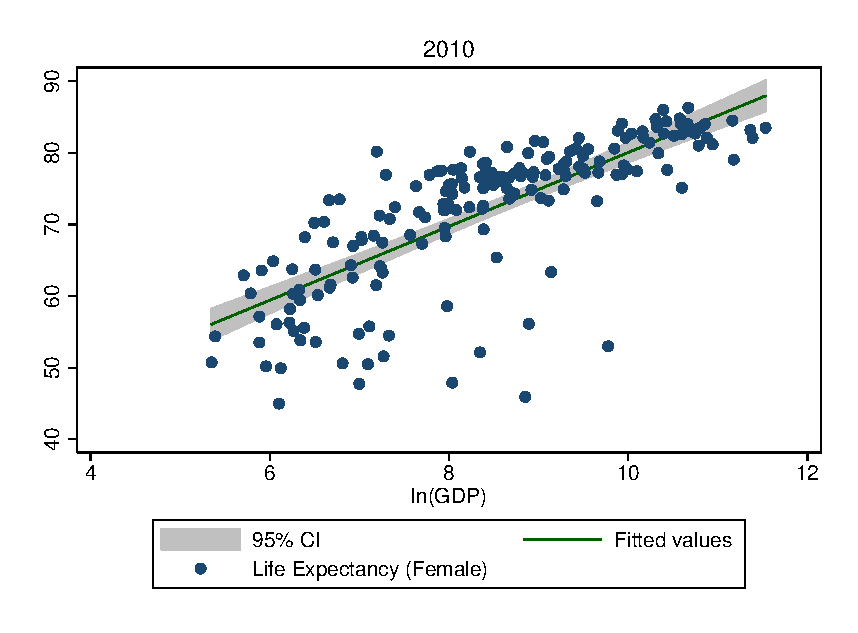
\includegraphics[scale= 0.22]{./../figures/lLEGDP2010}}
\caption{\footnotesize Female Life Expectancy is plotted  against log of GDP. The Life Expectancy (and the GDP) data comes from the World Bank WDI and spans over more than 190 countries and is available for the period of 1960 - 2011. Here we plot them for the years 1970, 1990 and 2010. \label{lLEGDP}}
\end{figure}

\begin{figure}[htpb!]
\centering
\subfloat[] {\includegraphics[scale= 0.22]{./../figures/lLErGDP1970}}
\subfloat[] {\includegraphics[scale= 0.22]{./../figures/lLErGDP1990}}
\subfloat[] {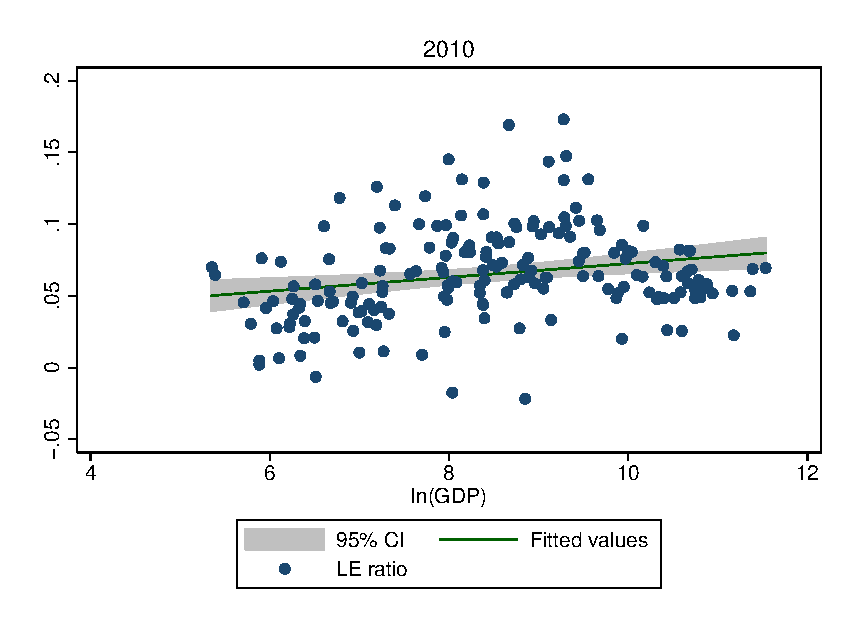
\includegraphics[scale= 0.22]{./../figures/lLErGDP2010}}
\caption{\footnotesize The log of the ratio of Female to Male Life Expectancy is plotted  against log of GDP. The Life Expectancy data comes from the World Bank WDI and spans over more than 190 countries and is available for the period of 1960 - 2011. Here we plot them for the years 1970, 1990 and 2010. \label{lLErGDP0}}
\end{figure}

\begin{figure}[htpb!]
\begin{center}
\includegraphics[scale=0.9]{./../figures/MMRRegion.eps} 
\caption{Maternal Mortality Ratio by Region: 1990-2010 (figure from \citet{BhalotraClarke2013})}
\label{fig:MMRRegion}
\end{center}
\end{figure}

\begin{figure}[htpb!]
\centering
\subfloat[] {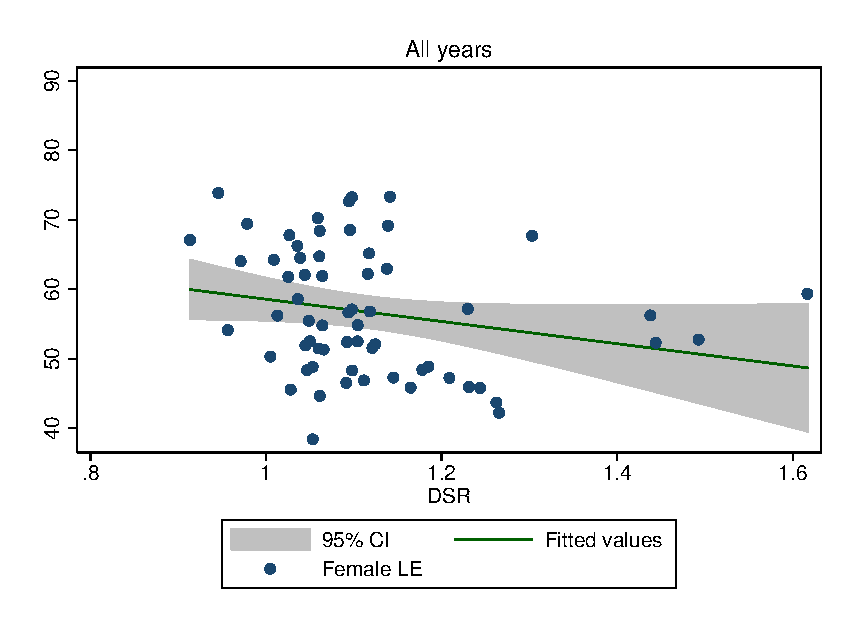
\includegraphics[scale= 0.25]{./../figures/lLEdesiredall}}
\subfloat[] {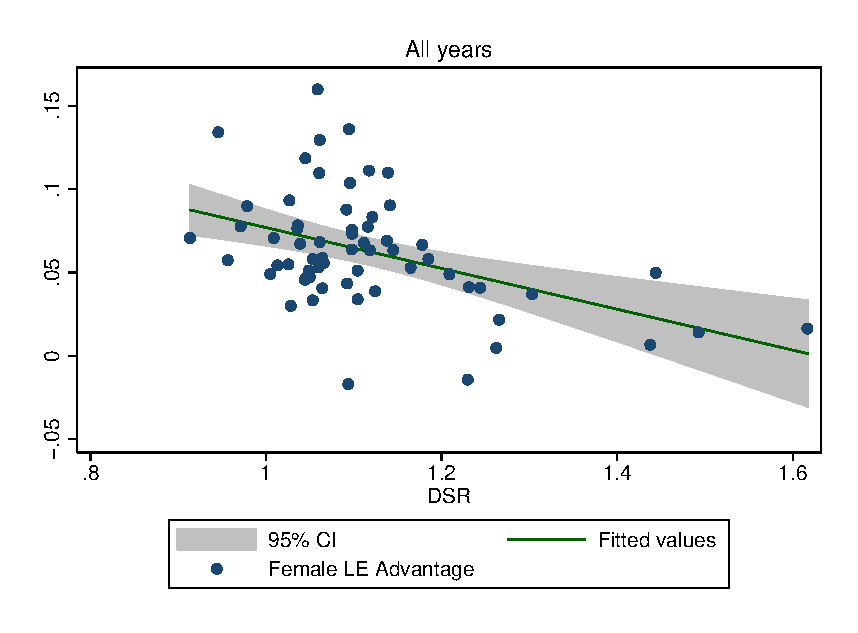
\includegraphics[scale= 0.25]{./../figures/lLErdesiredall}}
\caption{Female Life Expectancy is plotted against Desired Sex ratio (boys to girls). The Life Expectancy data comes from the World Bank WDI and spans over more than 190 countries and is available for the period of 1960 - 2011. Here we plot them for all years collapsed. The Desired Sex ratio (boys to girls) data is constructed from the DHS surveys which exists for 63 countries (mostly developing)}
\label{LFEgenderbias}
\end{figure}

\begin{figure}[htpb!]
\centering
\subfloat[] {\includegraphics[scale= 0.25]{./../figures/lMMRbDHSdesired2000}}
\subfloat[] {\includegraphics[scale= 0.25]{./../figures/lMMRbDHSdesired2010}}
\caption{MMR (per 100k births) from the DHS is plotted against Desired Sex ratio (boys to girls). The MMR data comes from a newly constructed database by Bhalotra et al. using the DHS sibling files. This data is based on the DHS sample (developing countries) of 45 countries and is available for the period of 1970 - 2012. Here we plot them for the DECADES 2000 and 2010. The Desired Sex ratio (boys to girls) data is constructed from the DHS surveys which exists for 63 countries (mostly developing).}
\label{MMRDgenderbias}
\end{figure}


\begin{figure}[htpb!]
\centering
\subfloat[] {\includegraphics[scale= 0.18]{./../figures/lMMRWDIdesired1990}}
\subfloat[] {\includegraphics[scale= 0.18]{./../figures/lMMRWDIdesired2000}}
\subfloat[] {\includegraphics[scale= 0.18]{./../figures/lMMRWDIdesired2010}}
\caption{MMR from WDI is plotted against Desired Sex ratio (boys to girls). The MMR data comes from World Bank WDI data which is based on data from WHO. It spans over around 180 countries from across the world and is available for 5 points of time - 1990, 1995, 2000, 2005, 2010. Here we plot data for three time periods, 1990, 2000, 2005. The Desired Sex ratio (boys to girls) data is constructed from the DHS surveys which exists for 63 countries (mostly developing). }
\label{MMRWgenderbias}
\end{figure}


\begin{figure}[htpb!]
\begin{center}
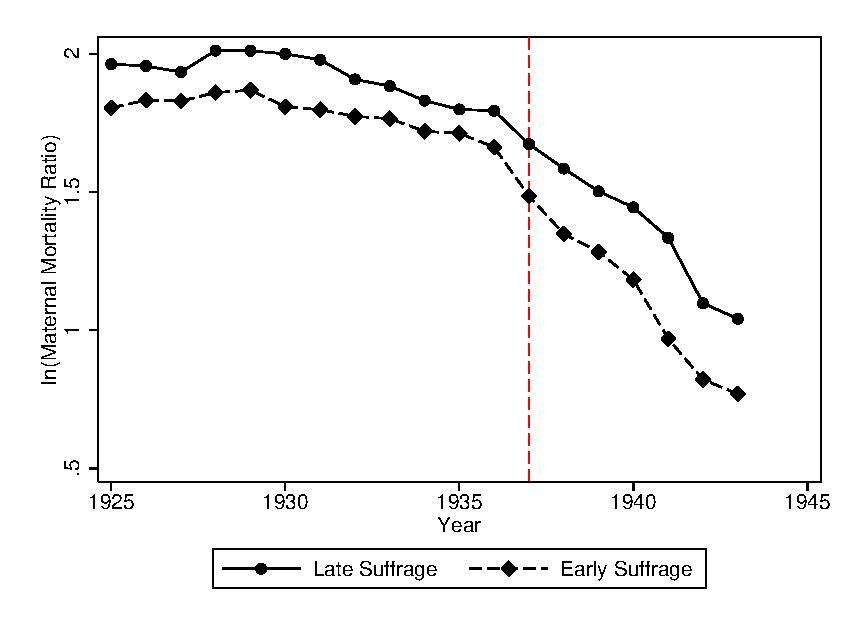
\includegraphics[scale=0.85]{../Source/atheen/MMRtrends.eps}
\caption{Trends in Maternal Mortality by Suffrage Type}
\label{trendMMR}
\end{center}
\end{figure}

\begin{figure}[htpb!]
\begin{center}
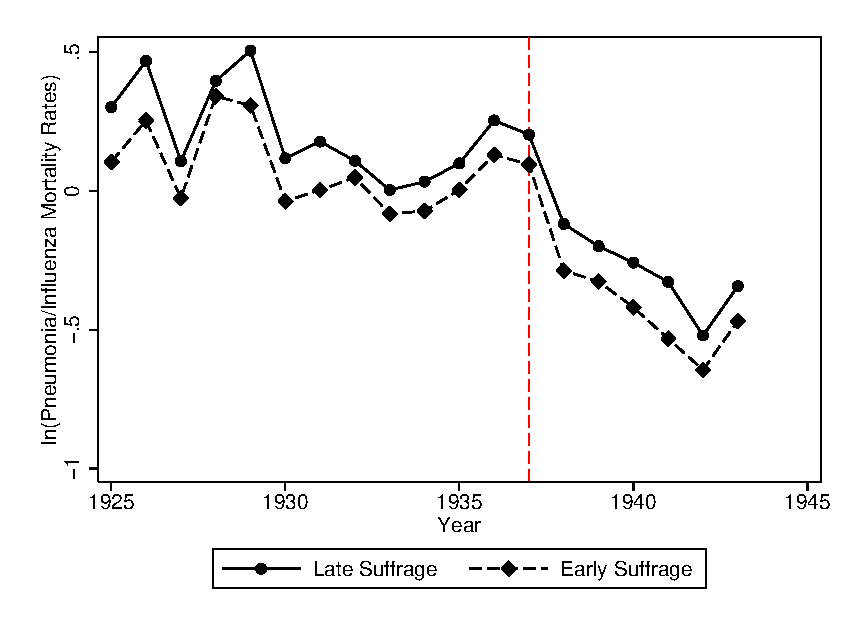
\includegraphics[scale=0.85]{../Source/atheen/IPRtrends.eps}
\caption{Trends in Pneumonia Mortality by Suffrage Type}
\label{trendIPR}
\end{center}
\end{figure}

\begin{figure}[htpb!]
\begin{center}
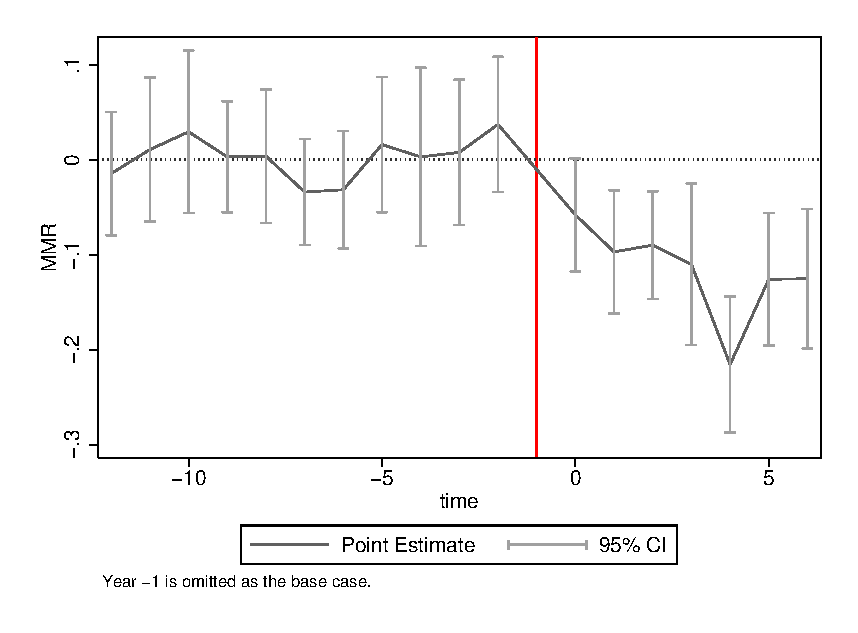
\includegraphics[scale=0.9]{../Source/atheen/eventMMR.eps}
\caption{Maternal Mortality Event Study Plot}
\label{eventMMR}
\end{center}
\end{figure}

\begin{figure}[htpb!]
\begin{center}
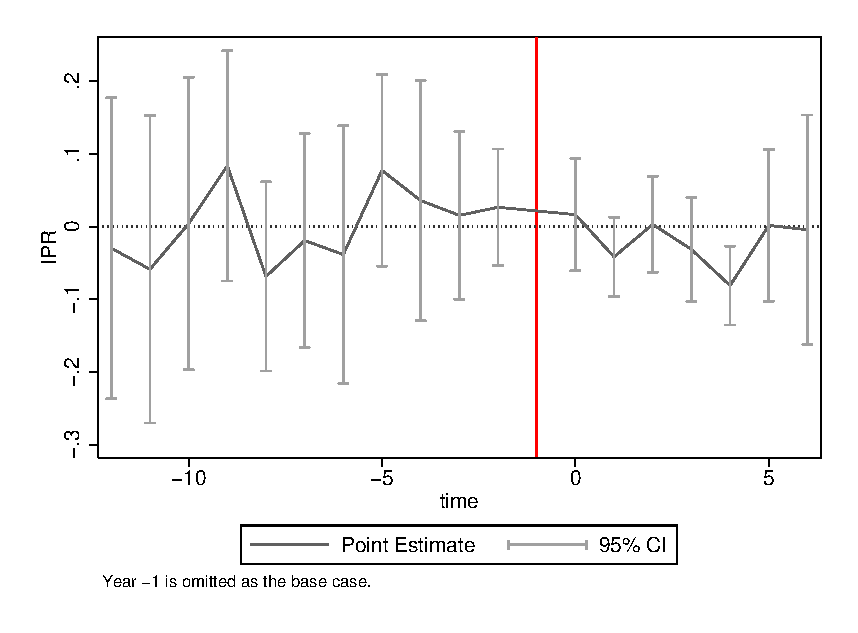
\includegraphics[scale=0.9]{../Source/atheen/eventIPR.eps}
\caption{Pneumonia (Placebo) Event Study Plot}
\label{eventIPR}
\end{center}
\end{figure}

\newpage
\section*{Tables}
\input{./../tables/sumStats.tex}
\begin{table}[htbp]\centering
\def\sym#1{\ifmmode^{#1}\else\(^{#1}\)\fi}
\caption{MMR and Desired Sex Ratio (boys/girls)}
\scalebox{0.7}{
\begin{tabular}{l*{5}{c}}
\toprule
                    &\multicolumn{1}{c}{(1)}   &\multicolumn{1}{c}{(2)}   &\multicolumn{1}{c}{(3)}   &\multicolumn{1}{c}{(4)}   &\multicolumn{1}{c}{(5)}   \\
                    &     MMR \ \   &     MMR \ \   &     MMR \ \   &     MMR \ \   &     MMR \ \   \\
\midrule
Desired Sex Ratio   &       824.7** &       655.0** &       667.0** &       923.9***&      2627.7***\\
                    &     [329.4]   &     [299.3]   &     [286.5]   &     [252.9]   &     [617.9]   \\
ln(GDP)             &               &               &        40.9   &        12.4   &       318.5***\\
                    &               &               &      [48.5]   &      [49.8]   &     [119.6]   \\
Desired Sex Ratio$\times$ ln(GDP)&               &               &               &               &      -285.3***\\
                    &               &               &               &               &     [100.7]   \\
Constant            &      -476.0   &      -405.1   &      -712.6   &     -1514.3***&     -3371.0***\\
                    &     [358.9]   &     [325.8]   &     [494.2]   &     [483.9]   &     [734.5]   \\
\midrule
R-squared           &        0.09   &        0.92   &        0.92   &        0.93   &        0.93   \\
Observations        &         310   &         310   &         307   &         307   &         307   \\
 Country FE &&Y&Y&Y&Y\\ Year FE&&Y&Y&Y&Y\\ 
Desired Fertility&&&&Y&Y\\
\bottomrule\end{tabular}}\end{table}

\input{./../Results/dsr/ln_LE_ratio-DSR.tex}
\input{./../Results/dsr/tb-DSR.tex}
\input{./../tables/rightsMMR.tex}
\input{./../tables/rightstb.tex}
\input{./../tables/rightsln_LE_ratio.tex}
\begin{landscape}
\input{./../tables/MMRGII.tex}
\end{landscape}
\begin{landscape}
\input{./../tables/ln_LE_ratioGII.tex}
\end{landscape}
\begin{landscape}
\begin{table}[htbp]\centering
\def\sym#1{\ifmmode^{#1}\else\(^{#1}\)\fi}
\caption{TB and Gender Intensity of Language Measures}
\scalebox{0.5}{
\begin{tabular}{l*{8}{c}}
\toprule
\textsc{Dep Var}:   &\multicolumn{1}{c}{(1)}&\multicolumn{1}{c}{(2)}&\multicolumn{1}{c}{(3)}&\multicolumn{1}{c}{(4)}&\multicolumn{1}{c}{(5)}&\multicolumn{1}{c}{(6)}&\multicolumn{1}{c}{(7)}&\multicolumn{1}{c}{(8)}\\
TB Incidence        &\multicolumn{1}{c}{NGII}&\multicolumn{1}{c}{SBII}&\multicolumn{1}{c}{GPII}&\multicolumn{1}{c}{GAII}&\multicolumn{1}{c}{GII0}&\multicolumn{1}{c}{GII1}&\multicolumn{1}{c}{GII2}&\multicolumn{1}{c}{GTroiano}\\
\midrule
\multicolumn{9}{l}{\textsc{Panel A: No Interaction}}\\
Gender Intensity Index&     -35.418*  &     -38.718   &     -70.779** &      19.500   &      -2.428   &       0.655   &     -23.346** &      -0.365   \\
                    &    [18.025]   &    [26.189]   &    [28.896]   &    [29.072]   &     [7.586]   &     [9.328]   &    [10.351]   &     [4.403]   \\
ln(GDP)             &     -40.202***&     -39.557***&     -49.045***&     -21.397** &     -21.940** &     -21.906** &     -38.367***&     -27.911***\\
                    &    [12.645]   &    [12.493]   &    [14.762]   &    [10.676]   &    [10.279]   &    [10.760]   &    [12.174]   &     [6.210]   \\
R-squared           &        0.55   &        0.55   &        0.52   &        0.58   &        0.57   &        0.57   &        0.56   &        0.55   \\
Observations        &        2619   &        2619   &        2561   &        1893   &        1812   &        1893   &        2469   &        1742   \\
\\ \multicolumn{9}{l}{\textsc{Panel B: GDP Interaction}}\\
Gender Intensity Index&    -113.987   &    -106.469   &    -212.387*  &      49.996   &      -5.372   &       2.209   &     -62.639*  &      15.251   \\
                    &    [80.285]   &    [88.634]   &   [109.688]   &   [151.564]   &    [34.552]   &    [44.033]   &    [36.067]   &    [22.170]   \\
GII $\times$ ln(GDP)&       9.411   &       8.485   &      17.487   &      -3.786   &       0.384   &      -0.204   &       5.032   &      -1.779   \\
                    &     [8.283]   &     [9.232]   &    [12.137]   &    [16.701]   &     [3.870]   &     [5.102]   &     [3.871]   &     [2.310]   \\
ln(GDP)             &     -44.724***&     -45.505***&     -54.743***&     -18.746   &     -22.978   &     -21.476   &     -46.338***&     -23.369***\\
                    &    [14.407]   &    [16.554]   &    [16.091]   &    [16.231]   &    [14.999]   &    [15.856]   &    [15.425]   &     [8.129]   \\
\midrule
R-squared           &        0.56   &        0.55   &        0.52   &        0.58   &        0.57   &        0.57   &        0.56   &        0.55   \\
Observations        &        2619   &        2619   &        2561   &        1893   &        1812   &        1893   &        2469   &        1742   \\
\bottomrule 
\end{tabular}}\end{table}

\end{landscape}
\input{./../tables/mechanism.tex}
\begin{landscape}
\input{./../Results/dsr/abortion-DSR.tex}
\end{landscape}\begin{landscape}
\input{./../tables/abortionGII.tex}
\end{landscape}
\input{./../tables/rightsabortionLeg.tex}


\newpage
\appendix
\section{Data Appendix}
\label{app:Data}
\subsection{\citet{CingranelliData2013} Data}
The women's political rights variable, takes into account women's right to vote, 
the right to run for political office, the right to hold elected and appointed 
government positions, the right to join political parties, and the right to petition 
government officials. 

The women's economic rights variable takes into account the rights to equal pay 
for equal work; free choice of profession or employment without the need to obtain 
a husband or male relative's consent; to gainful employment without the need to 
obtain a husband or male relative's consent; equality in hiring and promotion 
practices; job security (maternity leave, unemployment benefits, no arbitrary 
firing or layoffs, etc...); non-discrimination by employers; to be free from 
sexual harassment in the workplace; to work at night; to work in occupations 
classified as dangerous; to work in the military and the police force.  

And finally, the women's social rights include the rights to equal inheritance; 
to enter into marriage on a basis of equality with men; to travel abroad; to 
obtain a passport; to confer citizenship to children or a husband; to initiate a 
divorce; to own, acquire, manage, and retain property brought into marriage; to 
participate in social, cultural, and community activities; to an education; to 
choose a residence/domicile; freedom from female genital mutilation of children 
and of adults without their consent; and the freedom from forced sterilization.

All three of these variables take 4 discrete values of 0, 1, 2, and 3, with 
higher values indicating more rights for women. In addition we construct 2 other 
composite rights variables, the first one being the the first principal component 
of women's political, economic  and social rights and the second one only 
incorporates women's political and economic rights. Data on women's political 
and economic rights exists for the entire period of 1981- 2011, whereas data on 
women's social rights was discontinued after the year 2004 (see table 
\ref{RightsCount} for a full list of data availability by time.

%--------------------------------------------------------------------------------
\subsection{Gender Intensity of Language}
\citet{givati2012law} use the number of cases of gender differentiated pronouns 
for 33 languages (mostly but not entirely European) as a measure of gender 
neutrality of the language. According to their classification, the 33 languages 
can be divided into 4 distinct groups, with each group having either 0 (6 
languages), 1 (10 languages), 2 (14 languages), or 4 (3 languages) gender 
differentiated pronouns. Languages with a higher number of gender differentiated 
pronouns are supposed to be less gender neutral.

\cite{gay2013} construct measures from the World Atlas of Linguistic structures.
These are four binary variables related to gender neutrality of languages: 
Sex-Based Intensity Index, Number Gender Intensity Index, Gender Assignment 
Intensity Index, Gender Pronouns Intensity Index. Their final Gender Intensity 
index (GII) is a sum of all these four indices (or some combination of a subset 
of these indices). Since, all these four indices do not exist for all countries 
we sometimes choose a subset of these indices in order to maximize the number of 
observations. Suppose we choose to use three of these indices to construct our 
final Gender neutrality index, then $GII \in {0, 1, 2, 3}$ and all languages 
can be divided into 4 distinct classes of gender neutrality. For our final 
analysis we  use all eight of the following measures, the first seven of which 
come from \cite{gay2013} and the final one comes from \citet{givati2012law}.


\begin{enumerate}
\item Sex-Based Intensity Index (SBII) 
\item Number Gender Intensity Index (NGII)
\item Gender Assignment Intensity Index (GAII) 
\item Gender Pronouns Intensity Index (GPII) 
\item GII0 = NGII + SBII + GAII + GPII
\item GII1 = NGII + SBII + GAII
\item GII2 = NGII + SBII + GPII
\item gtroiano = number of cases of gender differentiated pronouns.
\end{enumerate}


%-------------------------------------------------------------------------------
\section{The Contribution of IMR and MMR to Gender Differences in Mortality}
In this section we quantify the contribution of maternal mortality and female to
 male infant mortality ratio to age specific mortality rates across genders. In 
previous studies, MMR has been found to contribute to female life expectancy. 
\citet{jayachandran2008life} show how a drop in MMR contributed to increased 
female life expectancy in Sri Lanka. \citet{canudas2014potential} estimate the 
contribution of maternal mortality to Reproductive-Aged Life Expectancy (RALE).
 They find that over the twentieth century, 5 years of RALE were gained in 
developed countries and around 10\% of this gain, or approximately half a year, 
can be attributed to reductions in Maternal mortality. ``In sub-Saharan African 
countries, the possible achievable gains fluctuate between 0.24 and 1.47 years, 
or 6\% and 44\% of potential gains in RALE'' \citep{canudas2014potential}.

Here, we establish that higher maternal mortality ratios can explain part of the 
excess female mortality in reproductive ages, which in turn explains part of the 
gender gap in life expectancy across countries. We first consider the differences 
in age specific mortality rates across genders and also the relative 
contributions of IMR and MMR (if any) to these mortality rates using data from UN 
mortality tables. In order to do so we consider 3 distinct age classes viz.\ 0-14, 
15-49 and 50+. The 15-49 age group is typically considered the reproductive age 
class for women and hence this is the class in which most maternal mortality 
should be concentrated. In order to compare differences between women and men, 
we construct the ratios of mortality rates of women to men in these three 
different age categories and use the log values of these ratios as our primary 
dependent variable.\footnote{Dependent variable = 
$\ln(\frac{\text{female mortality in age category X}}
{\text{male mortality in age category X}})*100000$; where X can be (0-14), 
(15-49), or, (50 +). This data comes from \citet{UNMortality2012}.}


Since this data exists for the entire world sample, we are able to analyze differences across countries belonging to the three different income categories of high, middle and low income countries following the World Bank's income classification. We thus regress the log ratio of female to male mortality rates (times 100,000) by different age categories on maternal mortality and infant mortality ratio for different countries in Table~\ref{MortalityMMRIncome}. In the three panels of Table~\ref{MortalityMMRIncome} we respectively have the low, middle and high income country samples.\footnote{See the appendix section~\ref{wblist} for a list of countries belonging to each of these categories.} In the odd numbered columns, we control for MMR and the log of GDP. In the even numbered columns we control for MMR, the log of GDP and the IMR ratio (female to male).\footnote{We include country fixed effects and time dummies in all columns and always use cluster robust standard errors clustered at the country level.}  

In Table~\ref{MortalityMMRIncome}, we first notice that for both the low and middle income category countries (i.e. in Panels 1 and 2), MMR significantly increases the excess female mortality for the 15-49 age category which is the reproductive age for women. This implies that some of the excess female to male mortality in the reproductive age is explained by MMR. In other words at least some of the 21\% of the 6 million women who are missing in their reproductive age every year around the world can be attributed to maternal mortality.\footnote{On the other hand, MMR significantly reduces excess female mortality in the 15-49 category and increases it in the 50+ category for high income countries. However, since MMR is concentrated solely in poorer countries, we cannot read too much into these numbers for developed countries.}\footnote{Both IMR and MMR are from the WDI and hence for the whole world sample. The IMR is available for 223 countries for the years 1990, 2000, 2010, 2012, while the MMR is available for 181 countries for the years 1990, 1995, 2000, 2005, 2010, and they have common data for 180 countries for the years 1990, 2000, and 2010. The 2 panels represent Low Income and Middle Income countries from the World Bank income group classification. There are 35 low income countries and 95 middle income countries according to this classification.  Again the female to male mortality ratios are available for the years 5 yearly from 1960 to 2005 and hence all these variables together are available only for the years 1990 and 2000. Hence there is a fall in observations from Col1 to Col2.} 


Let us now consider the marginal effects of our MMR variable (which is measured per 100,000 live births throughout the paper) on the log ratio of excess female mortality rates in the reproductive age. In order to do so we consider column 4 as our baseline specification. As far as the marginal effects for low income countries are concerned, a one s.d. (312.3) increase in MMR (measured as per 100,000 live births) leads to a 5.44\% (= (17.41*312.3)/100000) increase in the female to male mortality ratio in the reproductive age category. This is equivalent to 744\% (0.054/0.0073) of the mean of the female to male mortality in low income countries and around 35.78\% of the s.d. of the ratio of female to male mortality in this age category in these countries. For middle income countries on the other hand, a one s.d. (266.332) increase in MMR leads to a 4.29 (= (16.08*266.332)/100000) percentage points increase in the female to male mortality ratio in the reproductive age category. This is equivalent to a 14.03\% (0.043/0.305) decrease of the mean ratio of female to male mortality and around 13.67\% of the s.d. ratio of female to male mortality in this age category in these countries. The female to male infant mortality ratio on the other hand has no significant effect on the mortality rates in any of the three different age categories.\footnote{In the appendix Table~\ref{MortalityMMR} we provide a specification for the whole world sample pooled together.} In other words, if the average MMR in the low income countries in our sample which is around 451 in the year 2010, came down to the average MMR of the Middle income countries which is around 145 in the same year, then this fall of around 306 in the MMR would lead to a reduction in excess female mortality in the reproductive age by around 5\%. 

%In the above paragraphs we have established that MMR contributes to the excess female mortality in the reproductive ages of 15-49 in the low and middle income countries. Next, we study the contribution of MMR directly on female life expectancy advantage. Like the previous regression specifications, using a (country) Fixed Effects panel data framework with time dummies, in Table~\ref{FLEIMRWDIIncome} we regress the log ratio of female to male life expectancy on maternal mortality and the female to male infant mortality ratio from the WDI data for different regions of the world. Both life expectancy and MMR are measured as five yearly averages.  
%
%In the three panels of Table~\ref{FLEIMRWDIIncome} we respectively present the regression results for low, middle and high income category countries. We notice that maternal mortality reduces female advantage in life expectancy but this effect is not significant.\footnote{In the appendix Table~\ref{FLEIMRWDI} we provide a specification for the whole world sample pooled together.} 


%Considering column 6 as the baseline specification, we notice that a one s.d. (321.414) higher MMR implies about 7.71 decrease in the ratio of female advantage in life expectancy for our low income country sample of countries. This represents a 16.23\% of the mean and to around 25.03\% of the s.d. log life expectancy ratio of female to male for the low income country sample. \citet{canudas2014potential}on the other hand, find that the elimination of maternal mortality led to an increase of half a year of female reproductive age life expectancy (RALE) from 1930 to 1960 for industrialized countries. However, according to their calculations the gains in RALE from elimination of maternal mortality can range from as low as 0.24 years in Namibia to 1.47 years in Chad.\footnote{Female reproductive age life expectancy (RALE) is the female life expectancy calculated  from age 15 to 49 \citet{canudas2014potential}.}  

Let us now consider some individual country examples to see how different levels of MMR lead to different rates of life expectancy differences between women and men. If we consider India for example, which is a lower middle income country according to the World Bank income classification, the average MMR is 390 and the difference between female and male life expectancy is only of  0.59 years. Again, consider Nepal which also had a very high rate of MMR of 420 with the female advantage being only of 0.86 years. Again in Bangladesh, the MMR is around 466 and the women are actually at a disadvantage of 0.65 years. But, if we consider a country like Brazil which has roughly the same income level (upper middle income country) as India, they have a relatively low MMR rate of 84 and a female advantage in LE of 6.11 years. Similarly Thailand has an MMR of 55.2 and 6.07 years of female advantage. 


\newpage
\section{Appendix Figures}
\begin{figure}[h!]
\centering
\subfloat[] {\includegraphics[scale= 0.18]{./../figures/ScatterFLE_2010}}
\subfloat[] {\includegraphics[scale= 0.18]{./../figures/ScatterMLE_2010}}
\subfloat[] {\includegraphics[scale= 0.18]{./../figures/ScatterMLEr_2010}}
\caption{Female Life Expectancy (Panel 1, Male Life Expectancy (Panel 2) and Log(Female to Male Life Expectancy ratio) (Panel 3) is plotted against log of GDP. The Life Expectancy (and the GDP) data comes from the World Bank WDI and spans over more than 190 countries and is available for the period of 1960 - 2011. Here we plot them for the year 2010. \label{ScatterFLE}}
\end{figure}

\newpage
\section{Appendix Tables}
\input{./../Results/rights/MMR-WP.tex}
\input{./../Results/rights/ln_LE_ratio-WP.tex}
\input{./../Results/rights/tb-WP.tex}
\input{./../tables/rightsDesc.tex}
\begin{table}[h!]\centering
\def\sym#1{\ifmmode^{#1}\else\(^{#1}\)\fi}
\caption{Gender Differences in Mortality Rates \& Maternal Mortality}
\scalebox{0.6}{
\begin{tabular}{l*{6}{c}}
\toprule
            &\multicolumn{1}{c}{(1)}&\multicolumn{1}{c}{(2)}&\multicolumn{1}{c}{(3)}&\multicolumn{1}{c}{(4)}&\multicolumn{1}{c}{(5)}&\multicolumn{1}{c}{(6)}\\
            &\multicolumn{1}{c}{(0-14)}&\multicolumn{1}{c}{(0-14)}&\multicolumn{1}{c}{(15-49)}&\multicolumn{1}{c}{(15-49)}&\multicolumn{1}{c}{(50+)}&\multicolumn{1}{c}{(50+)}\\
\hline
Low Income\\
MMR         &      -4.640         &      -10.34\sym{*}  &       16.45\sym{***}&       17.41\sym{***}&      -2.515         &      -6.470         \\
            &     (4.637)         &     (5.286)         &     (4.701)         &     (5.284)         &     (3.886)         &     (5.586)         \\
lgdp     &     -1705.0         &     -5545.6\sym{*}  &      1928.7         &      3612.3         &      -325.6         &      -124.4         \\
            &    (1698.3)         &    (2750.4)         &    (2209.5)         &    (3482.2)         &    (1421.0)         &    (2152.0)         \\
IMR ratio (F/M)&                     &     -0.0723         &                     &      -1.511         &                     &       0.777         \\
            &                     &     (0.851)         &                     &     (1.153)         &                     &     (1.188)         \\
\hline
\(N\)       &         126         &          63         &         126         &          63         &         126         &          63         \\
r2          &       0.146         &       0.374         &       0.334         &       0.408         &       0.114         &       0.218         \\
\hline\hline
Middle Income\\
MMR         &      -8.961\sym{*}  &      -12.31\sym{**} &       17.90\sym{**} &       16.08\sym{**} &      -8.991\sym{*}  &      -7.516         \\
            &     (4.751)         &     (5.769)         &     (8.767)         &     (7.762)         &     (4.971)         &     (5.191)         \\
lgdp     &      2871.7\sym{**} &      1508.4         &     -2623.8         &     -5725.8\sym{**} &      -32.36         &       801.2         \\
            &    (1261.9)         &    (2059.6)         &    (1823.4)         &    (2339.8)         &     (678.2)         &    (1003.8)         \\
IMR ratio (F/M)&                     &       0.436         &                     &       1.066         &                     &      -0.731         \\
            &                     &     (0.481)         &                     &     (0.991)         &                     &     (0.490)         \\
\hline
\(N\)       &         368         &         183         &         368         &         183         &         368         &         183         \\
R$^2$          &      0.0717         &      0.0951         &       0.108         &       0.200         &      0.0537         &       0.103         \\
\bottomrule
\end{tabular}}
\end{table}





\end{spacing}
\end{document}



*POINT 1: 
